\documentclass[tikz,border=8pt]{standalone}
\usepackage{ctex}
\usepackage{amsmath,amssymb}
\usetikzlibrary{arrows.meta,calc,angles,quotes,positioning,decorations.pathmorphing,patterns}
\definecolor{ink}{RGB}{30,43,58}
\definecolor{blue}{RGB}{38,92,168}
\definecolor{orange}{RGB}{220,112,24}
\definecolor{green}{RGB}{38,139,93}
\definecolor{red}{RGB}{192,53,53}
\tikzset{
 line cap=round,line join=round,
 body/.style={draw=ink,very thick},
 axis/.style={-{Latex[length=2.5mm]},draw=ink,very thick},
 vec/.style={-{Latex[length=2.5mm]},draw=blue,very thick},
 force/.style={-{Latex[length=2.5mm]},draw=red,very thick},
 ray/.style={-{Latex[length=2.2mm]},draw=orange,very thick},
 guide/.style={draw=ink!48,dashed},
 dim/.style={{Latex[length=2mm]}-{Latex[length=2mm]},draw=ink!70}
}
\begin{document}

% question-01
\begin{tikzpicture}[scale=1]
 \coordinate (A) at (-2,-1.5); \coordinate (B) at (1.2,-1.5);
 \coordinate (C) at (2.2,-.35); \coordinate (D) at (-1,-.35);
 \coordinate (Ap) at (-2,.9); \coordinate (Bp) at (1.2,.9);
 \coordinate (Cp) at (2.2,2.05); \coordinate (Dp) at (-1,2.05);
 \fill[blue!7] (A)--(B)--(Bp)--(Ap)--cycle;
 \draw[body] (A)--(B)--(C)--(D)--cycle (Ap)--(Bp)--(Cp)--(Dp)--cycle;
 \draw[body] (A)--(Ap) (B)--(Bp) (C)--(Cp) (D)--(Dp);
 \foreach \p in {A,B,C,D,Ap,Bp,Cp,Dp}{\fill[ink] (\p) circle(2.5pt);}
 \node[red] at (-2.25,-1.75) {$\pm q$};
 \draw[dim] (-2,-2.05)--(1.2,-2.05) node[midway,below] {$l$};
 \fill[orange] (.1,.28) circle(2.5pt) node[right] {$O$};
 \node at (.1,-2.65) {八个等距顶点上的四个 $+q$ 与四个 $-q$};
\end{tikzpicture}

% solution-01
\begin{tikzpicture}[scale=.9]
 \begin{scope}[xshift=-4.5cm]
  \coordinate (A) at (-1.35,-.95); \coordinate (B) at (1.05,-.95);
  \coordinate (C) at (1.05,.95);   \coordinate (D) at (-1.35,.95);
  \coordinate (s) at (.65,.48);
  \draw[body] ($(A)+(s)$)--($(B)+(s)$)--($(C)+(s)$)--($(D)+(s)$)--cycle;
  \draw[body] (A)--(B)--(C)--(D)--cycle;
  \foreach \P in {A,B,C,D}{\draw[body] (\P)--($(\P)+(s)$);}
  \foreach \P in {A,B,C,D}{\fill[red] (\P) circle(3pt) node[left=2pt] {$+$};}
  \foreach \P in {A,B,C,D}{\fill[blue] ($(\P)+(s)$) circle(3pt) node[right=2pt] {$-$};}
  \draw[vec] (-.15,0)--(-2.65,0) node[left] {$\boldsymbol E_{\max}$};
  \node[align=center] at (0,-2.0) {相对两面分别放置\\四个正电荷与四个负电荷};
 \end{scope}
 \begin{scope}[xshift=1.0cm]
  \draw[axis] (0,0)--(3.7,0) node[right] {$|\boldsymbol U|^2$};
  \foreach \x/\lab in {0/0,.75/4,1.5/8,2.25/12,3.05/16}{
   \fill[blue] (\x,0) circle(2.8pt);
   \node[above=4pt] at (\x,0) {$\lab$};}
  \node[align=center] at (1.55,1.35) {允许的离散取值\\由顶点符号组合决定};
 \end{scope}
 \node[draw=ink!35,rounded corners,align=center,fill=white] at (1,-2.2)
 {$E=\dfrac{8kq}{3\sqrt3l^2}|\boldsymbol U|$\\[3pt]
  $|\boldsymbol U|^2\in\{0,4,8,12,16\}$};
\end{tikzpicture}

% question-02
\begin{tikzpicture}[scale=.92]
 \draw[guide] (0,2.7)--(0,-2.1) node[right] {向下竖直};
 \fill[ink] (0,2.7) circle(3pt) node[above] {$O$};
 \coordinate (A) at (-2.3,-1.2);
 \draw[body,line width=3pt] (0,2.7)--(A) node[midway,above left] {$l$};
 \draw[blue] (0,1.7) arc[start angle=-90,end angle=-121,radius=1.0];
 \node[blue] at (-.48,1.42) {$\theta$};
 \draw[body,fill=orange!8,rotate around={-31:(A)}] (A) ellipse(1.25 and .42);
 \draw[vec] ($(A)+(-.95,-.1)$) arc[start angle=195,end angle=450,x radius=.95,y radius=.28] node[right] {$\omega$};
 \fill[red] ($(A)+(-.15,.42)$) circle(3pt) node[above] {乘员};
 \node at (0,-3.0) {摆臂转轴、摆臂轴和圆环半径构成三维复合转动};
\end{tikzpicture}

% solution-02
\begin{tikzpicture}[scale=.78]
 \begin{scope}[xshift=-4.6cm]
  \fill[ink] (0,2.4) circle(3pt) node[above] {$O$};
  \coordinate (A) at (-1.5,-.8); \draw[body] (0,2.4)--(A);
  \draw[body,rotate around={-25:(A)}] (A) ellipse(.9 and .28);
  \coordinate (P) at (-1.68,-.48); \fill[red] (P) circle(3pt) node[above] {$P_{top}$};
  \draw[force] (A)--++(-125:1.45) node[below left] {$l\alpha_0$};
  \draw[vec] (P)--(A) node[midway,right] {$\omega^2r$};
  \node[align=center] at (0,-2.0) {$\Omega=0$\\$\boldsymbol a_P=\boldsymbol a_A-\omega^2\boldsymbol\rho$};
 \end{scope}
 \begin{scope}[xshift=3.4cm]
  \fill[ink] (0,2.4) circle(3pt) node[above] {$O$};
  \coordinate (A) at (0,-.6); \draw[body] (0,2.4)--(A);
  \draw[body] (A) ellipse(1.35 and .5);
  \coordinate (L) at (-1.35,-.6); \fill[red] (L) circle(3pt) node[left] {$P_L$};
  \draw[force] ($(A)+(.28,0)$)--++(90:1.2) node[right] {$\Omega^2l$};
  \draw[vec] (L)--(A) node[midway,below] {$\omega^2r$};
  \draw[green,very thick,-{Latex}] ($(A)+(-.28,0)$)--++(-90:1.25)
    node[midway,left=4pt] {$2\Omega\omega r$};
  \node[align=center] at (0,-2.75) {$\dot\Omega=0$\\科里奥利项沿摆臂轴};
 \end{scope}
\end{tikzpicture}

% question-03
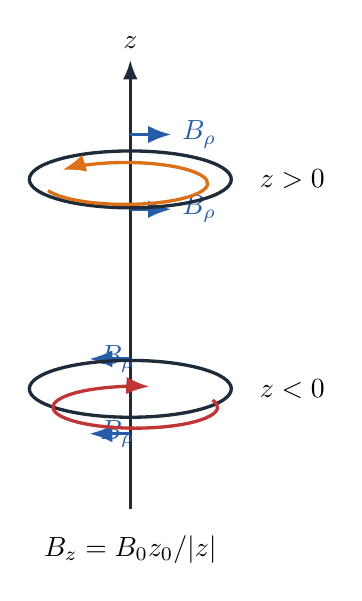
\begin{tikzpicture}[scale=.95]
 \draw[axis] (0,-3)--(0,3) node[above] {$z$};
 \foreach \z in {-2,-1,1,2}{
  \draw[blue,very thick,-{Latex}] (0,\z)--({.55*sign(\z)},\z) node[right] {$B_\rho$};}
 \draw[body] (0,1.4) ellipse(1.35 and .38);
 \draw[body] (0,-1.4) ellipse(1.35 and .38);
 \draw[orange,very thick,-{Latex}] (-1.1,1.25) arc[start angle=200,end angle=500,x radius=1.1,y radius=.28];
 \draw[red,very thick,-{Latex}] (1.1,-1.55) arc[start angle=20,end angle=-280,x radius=1.1,y radius=.28];
 \node[right] at (1.6,1.4) {$z>0$}; \node[right] at (1.6,-1.4) {$z<0$};
 \node at (0,-3.55) {$B_z=B_0z_0/|z|$};
\end{tikzpicture}

% solution-03
\begin{tikzpicture}[scale=.92]
 \draw[axis] (-3.2,0)--(3.4,0) node[right] {$z$};
 \draw[axis] (0,-2.0)--(0,3.2) node[above] {$F_z$};
 \draw[blue,very thick] plot[domain=.55:3,samples=80] (\x,{1.8/(\x*\x)});
 \draw[blue,very thick] plot[domain=-3:-.55,samples=80] (\x,{1.8/(\x*\x)});
 \draw[red,very thick] (-3,1.0)--(3,1.0) node[right] {$mg$};
 \draw[guide] (-1.34,0)--(-1.34,1.0); \draw[guide] (1.34,0)--(1.34,1.0);
 \fill[red] (-1.34,1) circle(3pt) node[above left] {$-a$ 不稳定};
 \fill[green] (1.34,1) circle(3pt) node[above right] {$+a$ 稳定};
 \node at (0,-2.55) {$a=\sqrt{\pi I B_0z_0r^2/(mg)}$};
\end{tikzpicture}

% question-04
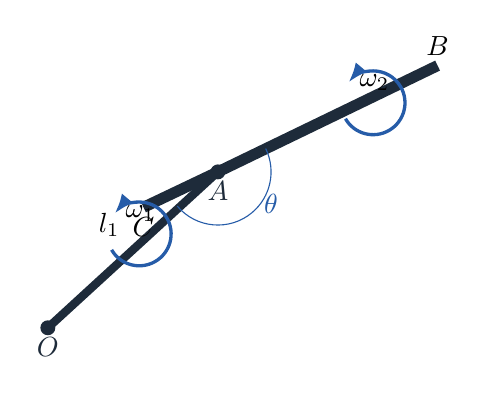
\begin{tikzpicture}[scale=.9]
 \fill[ink] (-3,-1.6) circle(3pt) node[below] {$O$};
 \coordinate (A) at (-.6,.6); \coordinate (B) at (2.5,2.1); \coordinate (C) at (-1.65,.1);
 \draw[body,line width=3pt] (-3,-1.6)--(A) node[midway,above left] {$l_1$};
 \draw[body,line width=4pt] (C)--(A)--(B);
 \fill[ink] (A) circle(3pt) node[below] {$A$}; \node[above] at (B) {$B$}; \node[below] at (C) {$C$};
 \draw[blue] (A)++(-140:.75) arc[start angle=-140,end angle=26,radius=.75];
 \node[blue] at (.15,.15) {$\theta$};
 \draw[vec] (-2.1,-.5) arc[start angle=210,end angle=500,radius=.45] node[right] {$\omega_1$};
 \draw[vec] (1.2,1.35) arc[start angle=210,end angle=500,radius=.45] node[right] {$\omega_2$};
\end{tikzpicture}

% solution-04
\begin{tikzpicture}[scale=.78]
 \coordinate (O) at (-4,-1.4); \coordinate (A) at (-1.6,.7); \coordinate (G) at (.2,1.35); \coordinate (B) at (2.0,2.0);
 \draw[body] (O)--(A); \draw[body,line width=4pt] (A)--(B);
 \fill[ink] (O) circle(3pt) node[below] {$O$}; \fill[ink] (A) circle(3pt) node[below right=3pt] {$A$}; \fill[orange] (G) circle(3pt) node[above] {$G$};
 \draw[orange,dashed,very thick,-{Latex}] (G)--++(205:1.55);
 \node[orange,above right=2pt] at (G) {$\boldsymbol a_G$};
 \draw[force] (A)--++(205:1.45) node[below left] {$\boldsymbol F_A=m\boldsymbol a_G$};
 \draw[red,very thick,-{Latex}] (A)++(.55,0) arc[start angle=0,end angle=275,radius=.55];
 \node[red] at (-.55,1.45) {$M_A$};
 \begin{scope}[xshift=5.0cm]
  \draw[body,line width=4pt] (-2.4,0)--(2.4,0);
  \fill[ink] (0,0) circle(3pt) node[below] {$A$};
  \fill[blue] (-1.55,0) circle(5pt) node[above] {$M$};
  \fill[orange] (1.2,0) circle(3pt) node[above] {$m$ 的质心};
  \draw[dim] (-1.55,-.55)--(0,-.55) node[midway,below] {$l_3$};
  \draw[dim] (0,-.55)--(1.2,-.55) node[midway,below] {$l_2/2$};
  \node at (0,-1.55) {$Ml_3=m l_2/2$};
 \end{scope}
\end{tikzpicture}

% question-05
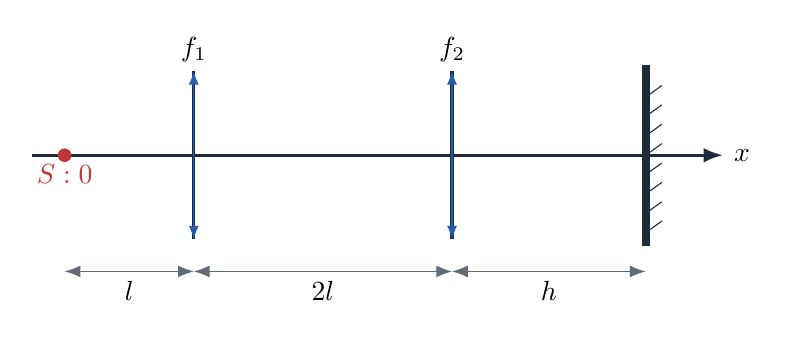
\begin{tikzpicture}[scale=.82]
 \draw[axis] (-.5,0)--(10.2,0) node[right] {$x$};
 \fill[red] (0,0) circle(3pt) node[below] {$S:0$};
 \foreach \x/\lab in {2/$f_1$,6/$f_2$}{
  \draw[body] (\x,-1.3)--(\x,1.3); \draw[blue,-{Latex}] (\x,0)--(\x,1.3); \draw[blue,-{Latex}] (\x,0)--(\x,-1.3); \node[above] at (\x,1.3) {\lab};}
 \draw[body,line width=3pt] (9,-1.4)--(9,1.4);
 \foreach \y in {-1.2,-.9,...,1.2}{\draw[ink] (9,\y)--(9.25,{\y+.18});}
 \draw[dim] (0,-1.8)--(2,-1.8) node[midway,below] {$l$};
 \draw[dim] (2,-1.8)--(6,-1.8) node[midway,below] {$2l$};
 \draw[dim] (6,-1.8)--(9,-1.8) node[midway,below] {$h$};
\end{tikzpicture}

% solution-05
\begin{tikzpicture}[scale=.72]
 \draw[axis] (-.4,0)--(15.55,0) node[above right] {展开坐标};
 \foreach \x/\lab in {2/$L_1$,6/$L_2$,8.8/$L_2'$,12.8/$L_1'$}{
  \draw[body] (\x,-1.05)--(\x,1.05); \node[above] at (\x,1.05) {\lab};}
 \fill[red] (0,0) circle(3pt) node[below] {$S$};
 \fill[red] (14.8,0) circle(3pt) node[below right] {$S'$};
 \draw[ray] (0,.55)--(2,.65)--(6,.25)--(8.8,-.15)--(12.8,-.5)--(14.8,0);
 \draw[ray] (0,-.35)--(2,-.2)--(6,.05)--(8.8,.2)--(12.8,.35)--(14.8,0);
 \draw[guide] (7.4,-1.45)--(7.4,1.45) node[above] {镜面展开线};
 \node[align=center] at (7.4,-2.0)
 {$M_{12}=0$\\
 $h'=\dfrac{f_2l(2l-3f_1)}{f_1f_2-3f_1l-f_2l+2l^2}$};
\end{tikzpicture}

% question-06
\begin{tikzpicture}[scale=.95]
 \draw[body] (0,0) circle(2.0);
 \draw[vec] (2,0) arc[start angle=0,end angle=255,radius=2];
 \fill[orange] (2,0) circle(4pt) node[right] {$\mu$};
 \foreach \x in {-2.6,-1.3,0,1.3,2.6}{\foreach \y in {-2.6,-1.3,0,1.3,2.6}{\node[blue] at (\x,\y) {$\times$};}}
 \node at (0,-3.25) {均匀磁场垂直纸面向里};
\end{tikzpicture}

% solution-06
\begin{tikzpicture}[scale=.9]
 \draw[axis] (0,0)--(6,0) node[right] {实验室时间};
 \draw[blue,very thick] (0,2.3)--(5.2,2.3);
 \draw[orange,very thick] (0,1.0)--(5.2,1.0);
 \draw[dim] (.2,2.65)--(2.6,2.65) node[midway,above] {$T_{lab}=\gamma\tau$};
 \draw[dim] (.2,.65)--(2.6,.65) node[midway,below] {$\tau_{lab}=\gamma\tau$};
 \foreach \x in {.2,2.6}{\draw[guide] (\x,.5)--(\x,2.8);}
 \node[align=center] at (3.8,1.65)
 {$T_{lab}/\tau_{lab}=1$\\一周后存活率仍为 $1/2$};
\end{tikzpicture}

% question-07
\begin{tikzpicture}[scale=.92]
 \draw[body,fill=blue!8] (-3,-1.7) rectangle (3,0);
 \draw[body,fill=ink!8] (-3,0)--(0,.65)--(3,0)--cycle;
 \node at (0,-.8) {室内 $T_1$}; \node at (0,.25) {屋顶};
 \foreach \x in {-2,-1,0,1,2}{\draw[ray] (\x,3)--(\x,.55);}
 \node[orange] at (2.6,2.55) {太阳 $I_0$};
 \draw[force] (-2.35,-.4)--(-2.35,-2.45) node[below] {$K(T_1-T_0)$};
 \draw[red,very thick,-{Latex}] (-.6,-.3)--(-.6,.7) node[left] {$\sigma T_1^4$};
 \draw[green,very thick,-{Latex}] (.6,.45)--(.6,-.45) node[right] {屋顶回辐射};
\end{tikzpicture}

% solution-07
\begin{tikzpicture}[scale=.78]
 \begin{scope}[xshift=-4.2cm]
  \node[draw,rounded corners,fill=orange!10,minimum width=4cm,minimum height=.9cm] (Sun) at (0,2.6) {太阳短波 $I_0$};
  \node[draw,rounded corners,fill=ink!7,minimum width=4cm,minimum height=.9cm] (Roof) at (0,.7) {传统屋顶 $r$};
  \node[draw,rounded corners,fill=blue!8,minimum width=4cm,minimum height=.9cm] (Room) at (0,-1.4) {室内黑体 $T_1$};
  \draw[ray] (Sun)--node[right] {吸收 $(1-r)I_0$}(Roof);
  \draw[red,very thick,<->] (Roof)--node[right] {长波交换}(Room);
 \end{scope}
 \begin{scope}[xshift=3.5cm]
  \node[draw,rounded corners,fill=orange!10,minimum width=4cm,minimum height=.9cm] (Sun2) at (0,2.6) {太阳短波};
  \node[draw,rounded corners,fill=green!8,minimum width=4cm,minimum height=.9cm] (Roof2) at (0,.7) {选择性屋顶};
  \node[draw,rounded corners,fill=blue!8,minimum width=4cm,minimum height=.9cm] (Room2) at (0,-1.4) {室内长波};
  \draw[ray] (Sun2)--node[right] {$1-r_H$}(Roof2);
  \draw[red,very thick,<->] (Roof2)--node[right] {$1-r_L$}(Room2);
  \node[align=center] at (0,-3.0) {$T_1=303.7\,\mathrm K$\\$T_1'=291.7\,\mathrm K$};
 \end{scope}
\end{tikzpicture}

% question-08
\begin{tikzpicture}[scale=.82]
 \fill[orange] (0,0) circle(7pt) node[below] {太阳};
 \draw[body] (0,0) circle(3.0);
 \draw[body] (0,0) circle(1.55);
 \draw[blue,very thick] (0,0) ellipse(3.0 and 1.55);
 \fill[blue] (3,0) circle(4pt) node[right] {地球};
 \fill[red] (-1.55,0) circle(3.5pt) node[left] {水星};
 \draw[ray] (3,.1)--(2.15,.65) node[above] {逆向点火};
 \node[blue] at (1.45,1.55) {转移椭圆};
\end{tikzpicture}

% solution-08
\begin{tikzpicture}[scale=.8]
 \begin{scope}[xshift=-4.3cm]
  \fill[orange] (0,0) circle(6pt) node[below] {太阳};
  \draw[body] (0,0) circle(2.5); \draw[body] (0,0) circle(1.25);
  \draw[blue,very thick] (0,0) ellipse(2.5 and 1.25);
  \fill[blue] (2.5,0) circle(3pt) node[right] {$v_E$};
  \draw[vec] (2.5,0)--(2.5,1.3) node[above] {$v_a$};
  \draw[force] (2.5,0)--(2.5,-.9) node[below] {$u_{\infty,E}=v_E-v_a$};
  \node[align=center] at (0,-3.05)
    {$v_0^2=u_{\infty,E}^2+2GM_E/R_E$};
 \end{scope}
 \begin{scope}[xshift=3.1cm]
  \fill[ink!15] (0,0) circle(1.2); \draw[body] (0,0) circle(1.2) node[below=1.3cm] {水星近场};
  \draw[guide] (0,0) circle(2.5);
  \draw[ray] (-3.2,1.6) .. controls (-2.1,1.2) and (-1.8,.4) .. (-1.2,0);
  \draw[vec] (-2.7,1.4)--(-1.8,1.0) node[above] {$u_\infty$};
  \draw[force] (-1.2,0)--(-.2,0) node[above] {$u_s$};
  \node[align=center] at (2.2,.4) {$u_s^2=u_\infty^2+2GM_M/R_M$\\$\Delta v\approx10.51\,\mathrm{km/s}$};
 \end{scope}
\end{tikzpicture}

\end{document}
